% ============================================================
%  Module 10 — Edinburgh's Legacy
%  From Smith to Simulation · University of Edinburgh
% ============================================================
\documentclass[aspectratio=169, 10pt]{beamer}
\usetheme{metropolis}

% --- Edinburgh colours ----------------------------------------
\definecolor{UoERed}{HTML}{7A2318}
\definecolor{UoEGold}{HTML}{B8860B}
\definecolor{CodeBG}{HTML}{F7F3ED}
\definecolor{CodeFrame}{HTML}{D5C9B1}

\setbeamercolor{palette primary}{bg=UoERed, fg=white}
\setbeamercolor{frametitle}{bg=UoERed, fg=white}
\setbeamercolor{title separator}{fg=UoEGold}
\setbeamercolor{progress bar}{fg=UoEGold, bg=UoEGold!20}
\setbeamercolor{alerted text}{fg=UoERed}
\setbeamercolor{block title}{bg=UoERed!15, fg=UoERed}
\setbeamercolor{block body}{bg=UoERed!5}

% --- Packages -------------------------------------------------
\usepackage[T1]{fontenc}
\usepackage{lmodern}
\usepackage{amsmath, amssymb, mathtools}
\usepackage{listings}
\usepackage{graphicx, booktabs}
\usepackage{tikz}
\usetikzlibrary{arrows.meta, positioning, calc, decorations.pathreplacing}
\usepackage{hyperref}
\hypersetup{colorlinks=true, linkcolor=UoERed, urlcolor=UoERed!70!black}
\setbeamertemplate{navigation symbols}{}

\lstset{
  language=Python,
  basicstyle=\ttfamily\scriptsize,
  keywordstyle=\color{UoERed}\bfseries,
  commentstyle=\color{gray}\itshape,
  stringstyle=\color{UoEGold},
  backgroundcolor=\color{CodeBG},
  frame=single,
  rulecolor=\color{CodeFrame},
  numbers=none,
  breaklines=true,
  showstringspaces=false,
  tabsize=4,
  xleftmargin=4pt, xrightmargin=4pt,
  aboveskip=6pt, belowskip=4pt,
}

% Section title pages
\AtBeginSection[]{
  \begin{frame}
    \vfill\centering
    \usebeamerfont{title}\insertsectionhead\par
    \vfill
  \end{frame}
}

% ---- Title ---------------------------------------------------
\title{Module 10 --- Edinburgh's Legacy}
\subtitle{Market Failures, Externalities, and the Future of Economics}
\author{Dr Juan Zurita}
\institute{From Smith to Simulation\\
The University of Edinburgh~$\cdot$~School of Economics}
\date{}

\begin{document}

% =============================================================
\maketitle
% =============================================================

% -------------------------------------------------------------
\section{Part I --- The History}
% -------------------------------------------------------------

\begin{frame}{Full Circle}
\begin{columns}[T]
\column{0.55\textwidth}
\begin{itemize}
  \item We began this course on the Royal Mile, in the Edinburgh of
        David Hume and Adam Smith.
  \item We end it there too --- but with \textbf{new eyes}.
  \item In the 1750s, Hume and Smith applied the methods of natural
        philosophy --- observation, systematic reasoning, scepticism ---
        to the study of human society.
  \item Their gift: the conviction that society is a \alert{natural system},
        governed by regularities discoverable through evidence.
\end{itemize}
\column{0.4\textwidth}
\begin{block}{The Method}
Observe the world carefully, build models that formalise your intuition,
test those models against data, and --- when the evidence demands it ---
change your mind.
\end{block}
\vspace{0.5em}
\textit{That is the Scottish Enlightenment's legacy to economics.}
\end{columns}
\end{frame}

\begin{frame}{The Arc of the Course (Weeks 1--5)}
\begin{description}
  \item[\textbf{Module 1: Smith}] Decentralised markets coordinate via the
        \textit{invisible hand}. We computed equilibrium by root-finding.
  \item[\textbf{Module 2: Ricardo \& Malthus}] Limits to growth --- scarcity
        shapes distribution. We simulated Malthusian dynamics and
        diminishing returns.
  \item[\textbf{Module 3: Keynes}] Markets do \textit{not} always clear ---
        demand failures cause unemployment. We built the multiplier model.
  \item[\textbf{Module 4: Marx}] Who benefits? Surplus value, capital
        accumulation, the falling labour share. We modelled CES production.
  \item[\textbf{Module 5: Marginalists}] Subjective utility replaces labour
        theory of value. We derived demand from optimisation.
\end{description}
\end{frame}

\begin{frame}{The Arc of the Course (Weeks 6--10)}
\begin{description}
  \item[\textbf{Module 6: Solow}] Capital accumulation and technological
        progress drive long-run growth. We simulated convergence to steady state.
  \item[\textbf{Module 7: Game Theory}] Strategic interaction --- payoffs
        depend on others' choices. We computed Nash equilibria.
  \item[\textbf{Module 8: Lucas}] Rational expectations and the Lucas critique.
        Policy works differently when agents anticipate it.
  \item[\textbf{Module 9: Piketty}] $r > g$: when returns on capital exceed
        growth, wealth concentrates across generations.
  \item[\textbf{Module 10: Today}] When does the invisible hand \alert{fail}?
        Market failures, externalities, and the future.
\end{description}
\end{frame}

\begin{frame}{The First Welfare Theorem}
Adam Smith's central claim, formalised:
\vspace{0.5em}
\begin{block}{First Welfare Theorem}
Under \textbf{perfect competition}, with \textbf{no externalities} and
\textbf{complete information}, the competitive equilibrium is
\textbf{Pareto efficient} --- no one can be made better off without
making someone worse off.
\end{block}
\vspace{0.5em}
But those conditions are \alert{demanding}. Today we run three
computational experiments that each violate one condition:
\begin{enumerate}
  \item \textbf{Externalities} --- pollution (violates ``no externalities'')
  \item \textbf{Asymmetric information} --- Akerlof's lemons
  \item \textbf{Market power} --- monopoly (violates ``perfect competition'')
\end{enumerate}
\vspace{0.3em}
In each case, we compute the gap between what the market delivers
and what society needs.
\end{frame}

\begin{frame}{Market Failures as Challenges to Smith}
\begin{center}
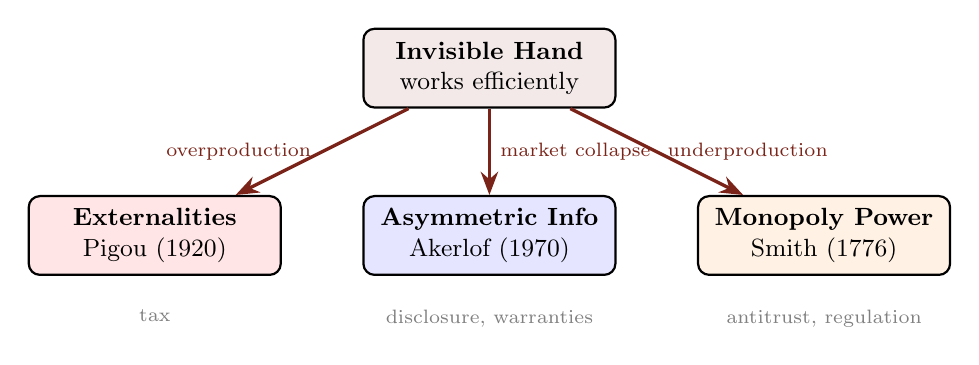
\begin{tikzpicture}[>=Stealth, thick, scale=0.85,
    box/.style={draw, rounded corners, minimum width=3.2cm,
                minimum height=1cm, font=\small, align=center}]
  \node[box, fill=UoERed!10] (ih) at (0,0)
    {\textbf{Invisible Hand}\\works efficiently};
  \node[box, fill=red!10] (ext) at (-5,-2.5)
    {\textbf{Externalities}\\Pigou (1920)};
  \node[box, fill=blue!10] (info) at (0,-2.5)
    {\textbf{Asymmetric Info}\\Akerlof (1970)};
  \node[box, fill=orange!10] (mono) at (5,-2.5)
    {\textbf{Monopoly Power}\\Smith (1776)};
  \draw[->, UoERed, line width=1.2pt] (ih) -- (ext)
    node[midway, left, font=\scriptsize] {overproduction};
  \draw[->, UoERed, line width=1.2pt] (ih) -- (info)
    node[midway, right, font=\scriptsize] {market collapse};
  \draw[->, UoERed, line width=1.2pt] (ih) -- (mono)
    node[midway, right, font=\scriptsize] {underproduction};
  \node[below=0.3cm of ext, font=\scriptsize, text=gray] {tax};
  \node[below=0.3cm of info, font=\scriptsize, text=gray]
    {disclosure, warranties};
  \node[below=0.3cm of mono, font=\scriptsize, text=gray]
    {antitrust, regulation};
\end{tikzpicture}
\end{center}
\end{frame}

\begin{frame}{Externalities: Pigou's Correction}
\begin{columns}[T]
\column{0.55\textwidth}
\begin{itemize}
  \item A \textbf{negative externality} is a cost imposed on third parties
        who are not part of the market transaction.
  \item Example: a factory on the Water of Leith produces cloth but
        pollutes the river, harming fishermen and residents downstream.
  \item The factory ignores these costs $\Rightarrow$ it produces
        \alert{too much}.
  \item \textbf{Arthur Pigou} (1877--1959): a tax equal to the marginal
        external cost can restore efficiency.
\end{itemize}
\column{0.4\textwidth}
\begin{block}{Key Distinction}
\begin{description}
  \item[PMC] Private marginal cost\\(what the firm pays)
  \item[EMC] External marginal cost\\(the pollution damage)
  \item[SMC] Social marginal cost\\$= PMC + EMC$
\end{description}
\end{block}
\end{columns}
\end{frame}

\begin{frame}{Information Asymmetry: Akerlof's Lemons}
\begin{itemize}
  \item George Akerlof, ``The Market for `Lemons'\,'' \textit{QJE} (1970).
        Nobel Prize 2001.
  \item \textbf{Setup:} sellers know the quality of their used cars;
        buyers cannot observe it.
  \item Buyers offer a price reflecting \textit{average} quality.
  \item Sellers of \textit{good} cars find this price too low
        $\Rightarrow$ they \alert{withdraw}.
  \item Average quality drops $\Rightarrow$ price drops further
        $\Rightarrow$ more good cars leave.
  \item \textbf{Adverse selection spiral}: only ``lemons'' remain.
\end{itemize}
\vspace{0.5em}
\begin{alertblock}{Real-world consequences}
Vehicle history reports, health insurance mandates, warranties,
and certifications all exist to combat this market failure.
\end{alertblock}
\end{frame}

\begin{frame}{Monopoly: Smith's Original Warning}
\begin{center}
\textit{``The price of monopoly is upon every occasion the highest
which can be got. The natural price, or the price of free competition,
\ldots\ is the lowest which can be taken.''}\\[4pt]
--- Adam Smith, \textit{The Wealth of Nations}, Book~I, Ch.~7
\end{center}
\vspace{0.5em}
\begin{itemize}
  \item A monopolist restricts output and raises price above marginal cost.
  \item Consumer surplus falls; part is captured as monopoly profit,
        part is \alert{deadweight loss} --- pure waste.
  \item Smith understood this in 1776. Two and a half centuries later,
        the same logic drives antitrust enforcement against tech giants.
\end{itemize}
\end{frame}

\begin{frame}{The Frontier Today}
\begin{columns}[T]
\column{0.48\textwidth}
\begin{block}{Climate Economics}
Nordhaus's DICE model integrates climate science with growth theory.
Draws on Solow (growth), Piketty (distribution), marginalists
(optimisation).
\end{block}
\vspace{0.3em}
\begin{block}{AI and Automation}
The ``machinery question'' of Ricardo and Marx returns. CES production
(Module~4) is precisely the tool economists use.
\end{block}
\column{0.48\textwidth}
\begin{block}{Agent-Based Models}
Simulate millions of heterogeneous agents interacting. Smith's invisible
hand made literal: outcomes \textit{emerge} from decentralised
interaction.
\end{block}
\vspace{0.3em}
\begin{block}{Machine Learning in Economics}
Causal inference and high-dimensional data transform empirical economics.
The Scottish emphasis on evidence has never been more relevant.
\end{block}
\end{columns}
\end{frame}

\begin{frame}{Edinburgh's Continuing Legacy}
\begin{itemize}
  \item The University of Edinburgh remains at the frontier: inequality,
        development, behavioural economics, computational methods.
  \item The city that gave the world Hume's scepticism and Smith's
        invisible hand continues to shape how we understand economic life.
  \item And the method remains the same:
\end{itemize}
\vspace{0.5em}
\begin{center}
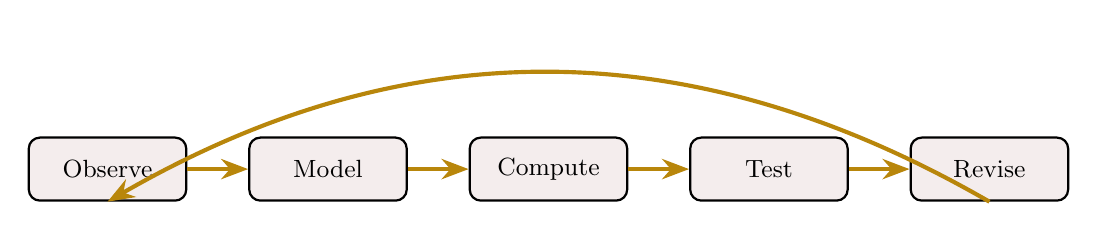
\begin{tikzpicture}[>=Stealth, thick,
    mstep/.style={draw, rounded corners, fill=UoERed!8,
                  minimum width=2cm, minimum height=0.8cm, font=\small}]
  \node[mstep] (obs) at (0,0) {Observe};
  \node[mstep] (mod) at (2.8,0) {Model};
  \node[mstep] (comp) at (5.6,0) {Compute};
  \node[mstep] (test) at (8.4,0) {Test};
  \node[mstep] (rev) at (11.2,0) {Revise};
  \draw[->, UoEGold, line width=1.5pt] (obs) -- (mod);
  \draw[->, UoEGold, line width=1.5pt] (mod) -- (comp);
  \draw[->, UoEGold, line width=1.5pt] (comp) -- (test);
  \draw[->, UoEGold, line width=1.5pt] (test) -- (rev);
  \draw[->, UoEGold, line width=1.5pt, bend right=30] (rev.south) to (obs.south);
\end{tikzpicture}
\end{center}
\vspace{0.3em}
\begin{center}
\textit{Hume's scepticism made operational: don't trust your
assumptions --- test them.}
\end{center}
\end{frame}

% -------------------------------------------------------------
\section{Part II --- The Computation}
% -------------------------------------------------------------

\begin{frame}[fragile]{Setting Up}
\begin{lstlisting}
import numpy as np
import matplotlib.pyplot as plt
from scipy.optimize import minimize, fsolve
\end{lstlisting}
\vspace{0.5em}
\begin{itemize}
  \item \texttt{numpy} --- numerical arrays and operations
  \item \texttt{matplotlib} --- plotting
  \item \texttt{fsolve} --- root-finding (equilibrium as $ED = 0$)
  \item \texttt{minimize} --- optimisation (monopolist's problem)
\end{itemize}
\vspace{0.3em}
Today we put the invisible hand on trial with three computational
experiments.
\end{frame}

\begin{frame}{Model 1: The Polluting Factory}
A factory on the Water of Leith produces cloth. Production generates
pollution that harms downstream residents.
\vspace{0.5em}
\begin{align*}
  PMC(Q) &= 2 + 0.1\,Q & &\text{(Private marginal cost)} \\[4pt]
  EMC(Q) &= 0.05\,Q & &\text{(External marginal cost)} \\[4pt]
  SMC(Q) &= 2 + 0.15\,Q & &\text{(Social marginal cost)} \\[4pt]
  P(Q) &= 20 - 0.2\,Q & &\text{(Demand)}
\end{align*}
\vspace{0.3em}
\begin{itemize}
  \item \textbf{Free market:} set $P = PMC$ (factory ignores pollution).
  \item \textbf{Social optimum:} set $P = SMC$ (society accounts for pollution).
  \item The gap is the market failure.
\end{itemize}
\end{frame}

\begin{frame}[fragile]{Computing the Externality Equilibria}
\begin{lstlisting}
def demand(Q):    return 20 - 0.2 * Q
def PMC(Q):       return 2 + 0.1 * Q
def EMC(Q):       return 0.05 * Q
def SMC(Q):       return PMC(Q) + EMC(Q)

# Free-market: demand = PMC
# 20 - 0.2Q = 2 + 0.1Q => Q = 60
Q_market = fsolve(lambda Q: demand(Q) - PMC(Q), 30)[0]

# Social optimum: demand = SMC
# 20 - 0.2Q = 2 + 0.15Q => Q = 51.43
Q_social = fsolve(lambda Q: demand(Q) - SMC(Q), 30)[0]

# Pigouvian tax = EMC at social optimum
pigouvian_tax = EMC(Q_social)   # 2.57 per unit
\end{lstlisting}
\vspace{0.3em}
The free market overproduces by $60 - 51.4 \approx 8.6$ units.
\end{frame}

\begin{frame}{Externality: Social vs Private Optimum}
\begin{center}
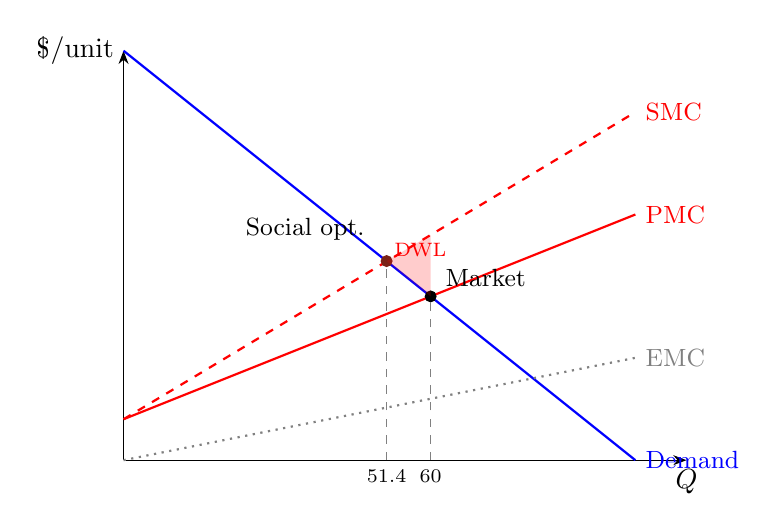
\begin{tikzpicture}[scale=0.65, >=Stealth]
  % Axes
  \draw[->] (0,0) -- (11,0) node[below] {$Q$};
  \draw[->] (0,0) -- (0,8) node[left] {\$/unit};
  % Scale: Q 0-100 => 0-10, P 0-20 => 0-8
  % Demand: P = 20 - 0.2Q. At Q=0 P=20 (y=8), at Q=100 P=0 (x=10)
  \draw[thick, blue] (0,8) -- (10,0) node[right, font=\small] {Demand};
  % PMC: P = 2 + 0.1Q. At Q=0 P=2 (y=0.8), at Q=100 P=12 (y=4.8)
  \draw[thick, red] (0,0.8) -- (10,4.8) node[right, font=\small] {PMC};
  % SMC: P = 2 + 0.15Q. At Q=0 P=2 (y=0.8), at Q=100 P=17 (y=6.8)
  \draw[thick, red, dashed] (0,0.8) -- (10,6.8) node[right, font=\small] {SMC};
  % EMC: P = 0.05Q. At Q=0 P=0, at Q=100 P=5 (y=2)
  \draw[thick, gray, dotted] (0,0) -- (10,2) node[right, font=\small] {EMC};
  % Market eq: Q=60 (x=6), P_mkt = 20 - 12 = 8 (y=3.2)
  \filldraw (6, 3.2) circle (3pt);
  \node[above right, font=\small] at (6.1, 3.2) {Market};
  % Social opt: Q=51.43 (x=5.14), P_soc = 20 - 10.29 = 9.71 (y=3.89)
  \filldraw[UoERed] (5.14, 3.89) circle (3pt);
  \node[above left, font=\small] at (4.9, 4.1) {Social opt.};
  % DWL shading: between demand and SMC from Q_social to Q_market
  % At Q_social (5.14): demand=3.89, SMC=3.89 (they meet)
  % At Q_market (6): demand=3.2, SMC=2+0.15*60=11 => y=4.4
  \fill[red, opacity=0.2] (5.14,3.89) -- (6,3.2) -- (6,4.4) -- cycle;
  \node[font=\scriptsize, text=red] at (5.8, 4.1) {DWL};
  % Dashed lines
  \draw[dashed, gray] (5.14,0) -- (5.14,3.89);
  \draw[dashed, gray] (6,0) -- (6,3.2);
  \node[below, font=\scriptsize] at (5.14,0) {$51.4$};
  \node[below, font=\scriptsize] at (6,0) {$60$};
\end{tikzpicture}
\end{center}
\vspace{0.3em}
Every unit between $Q_{\text{social}}$ and $Q_{\text{market}}$ costs society
more (SMC) than it benefits consumers (demand). The shaded triangle is the
\alert{deadweight loss} from the externality.
\end{frame}

\begin{frame}{The Pigouvian Tax}
\begin{block}{Corrective Policy}
A \textbf{Pigouvian tax} $\tau^* = EMC(Q^*_{\text{social}}) \approx 2.57$
per unit shifts the private cost curve up so that
$PMC(Q) + \tau^* = SMC(Q)$ at the optimum.
\end{block}
\vspace{0.5em}
\begin{itemize}
  \item Named after \textbf{Arthur Pigou} (1877--1959), a student of
        Alfred Marshall at Cambridge.
  \item The tax ``internalises the externality'' --- the polluter now
        faces the \textit{full} social cost.
  \item Deadweight loss:
  \[
    DWL = \tfrac{1}{2}(Q_{\text{mkt}} - Q_{\text{soc}})
          \bigl(SMC(Q_{\text{mkt}}) - P(Q_{\text{mkt}})\bigr)
        \approx 12.86
  \]
  \item This is the gain from imposing the carbon tax.
\end{itemize}
\end{frame}

\begin{frame}{Model 2: Akerlof's Market for Lemons}
\begin{columns}[T]
\column{0.55\textwidth}
\begin{itemize}
  \item $n = 10{,}000$ used cars, quality $q \sim U[0,1]$.
  \item Seller values car at $q$; buyer values it at $1.5\,q$
        (gains from trade exist for every car).
  \item But the buyer \alert{cannot observe} $q$.
  \item Buyer offers price $= 1.5 \times \bar{q}$
        (expected quality of cars on the market).
  \item Sellers with $q > \text{price}$ withdraw.
\end{itemize}
\column{0.4\textwidth}
\begin{center}
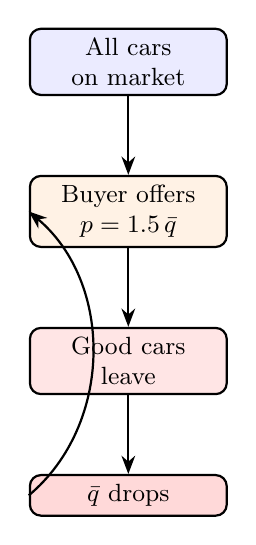
\begin{tikzpicture}[>=Stealth, thick, scale=0.8]
  \node[draw, rounded corners, fill=blue!8, font=\small,
        minimum width=2.5cm, align=center] (start)
    {All cars\\on market};
  \node[draw, rounded corners, fill=orange!10, font=\small,
        minimum width=2.5cm, align=center, below=1cm of start] (offer)
    {Buyer offers\\$p = 1.5\,\bar{q}$};
  \node[draw, rounded corners, fill=red!10, font=\small,
        minimum width=2.5cm, align=center, below=1cm of offer] (leave)
    {Good cars\\leave};
  \node[draw, rounded corners, fill=red!15, font=\small,
        minimum width=2.5cm, align=center, below=1cm of leave] (drop)
    {$\bar{q}$ drops};
  \draw[->] (start) -- (offer);
  \draw[->] (offer) -- (leave);
  \draw[->] (leave) -- (drop);
  \draw[->, bend right=50] (drop.west) to (offer.west);
\end{tikzpicture}
\end{center}
\end{columns}
\end{frame}

\begin{frame}[fragile]{Simulating Adverse Selection}
\begin{lstlisting}
def lemons_market(n_cars=10000, buyer_premium=1.5, seed=42):
    rng = np.random.default_rng(seed)
    qualities = rng.uniform(0, 1, n_cars)
    on_market = np.ones(n_cars, dtype=bool)

    for round_num in range(1, 51):
        if on_market.sum() == 0:
            break
        avg_q = qualities[on_market].mean()
        price = buyer_premium * avg_q
        new_on = on_market & (qualities <= price)
        if np.array_equal(new_on, on_market):
            break
        on_market = new_on
    return qualities, on_market
\end{lstlisting}
\vspace{0.3em}
With \textbf{full information}: all 10\,000 cars trade.\\
With \textbf{asymmetric information}: only lemons remain --- the market
has \alert{partially collapsed}.
\end{frame}

\begin{frame}{The Adverse Selection Spiral}
\begin{center}
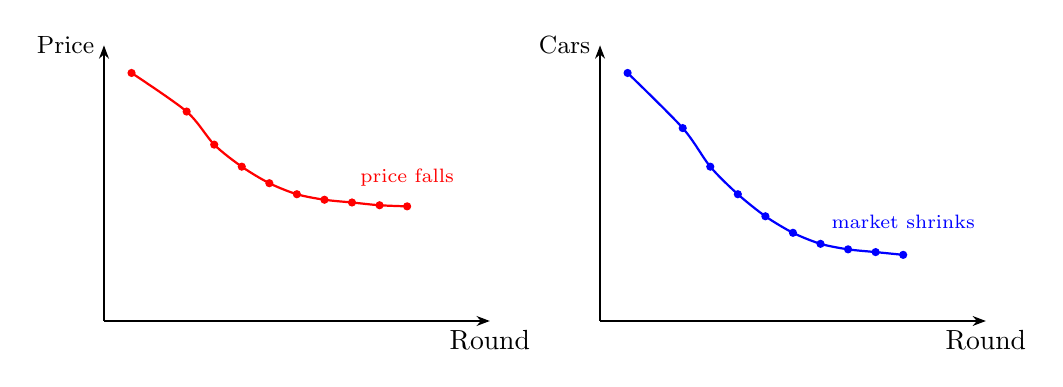
\begin{tikzpicture}[scale=0.7, >=Stealth]
  % Price panel
  \draw[->] (0,0) -- (7,0) node[below] {Round};
  \draw[->] (0,0) -- (0,5) node[left, font=\small] {Price};
  \draw[thick, red] plot[smooth, mark=*, mark size=1.5pt] coordinates
    {(0.5,4.5) (1.5,3.8) (2,3.2) (2.5,2.8) (3,2.5) (3.5,2.3) (4,2.2)
     (4.5,2.15) (5,2.1) (5.5,2.08)};
  \node[font=\scriptsize, red] at (5.5,2.6) {price falls};
  % Cars panel
  \begin{scope}[xshift=9cm]
  \draw[->] (0,0) -- (7,0) node[below] {Round};
  \draw[->] (0,0) -- (0,5) node[left, font=\small] {Cars};
  \draw[thick, blue] plot[smooth, mark=*, mark size=1.5pt] coordinates
    {(0.5,4.5) (1.5,3.5) (2,2.8) (2.5,2.3) (3,1.9) (3.5,1.6) (4,1.4)
     (4.5,1.3) (5,1.25) (5.5,1.2)};
  \node[font=\scriptsize, blue] at (5.5,1.8) {market shrinks};
  \end{scope}
\end{tikzpicture}
\end{center}
\vspace{0.5em}
\begin{center}
Low price $\;\to\;$ good cars leave $\;\to\;$ quality drops $\;\to\;$
lower price $\;\to\;$ \ldots\\[6pt]
\textit{The invisible hand cannot work when one side of the market is blind.}
\end{center}
\end{frame}

\begin{frame}{Model 3: Monopoly vs Competition}
Market with inverse demand $P(Q) = 20 - 0.2\,Q$ and constant
marginal cost $MC = 4$.
\vspace{0.5em}
\begin{columns}[T]
\column{0.48\textwidth}
\begin{block}{Perfect Competition}
Many firms, price-takers: $P = MC$
\[
  20 - 0.2\,Q = 4 \implies Q_c = 80,\ P_c = 4
\]
\end{block}
\column{0.48\textwidth}
\begin{block}{Monopoly}
Single firm maximises $\pi = (P - MC)\,Q$\\
$MR = 20 - 0.4\,Q$; set $MR = MC$:
\[
  20 - 0.4\,Q = 4 \implies Q_m = 40,\ P_m = 12
\]
\end{block}
\end{columns}
\vspace{0.5em}
\begin{itemize}
  \item Monopoly profit: $(12 - 4)\times 40 = 320$
  \item Deadweight loss: $\tfrac{1}{2}(80 - 40)(12 - 4) = \alert{160}$
\end{itemize}
\end{frame}

\begin{frame}[fragile]{Computing Monopoly vs Competition}
\begin{lstlisting}
MC = 4

def inverse_demand(Q): return 20 - 0.2 * Q
def marginal_revenue(Q): return 20 - 0.4 * Q

# Competitive: P = MC
Q_comp = fsolve(lambda Q: inverse_demand(Q) - MC, 50)[0]

# Monopoly: MR = MC
Q_mono = fsolve(lambda Q: marginal_revenue(Q) - MC, 30)[0]
P_mono = inverse_demand(Q_mono)

# Deadweight loss
DWL = 0.5 * (Q_comp - Q_mono) * (P_mono - MC)  # 160
profit = (P_mono - MC) * Q_mono                 # 320
\end{lstlisting}
\vspace{0.3em}
The monopolist restricts output by 40 units and raises price by 8.\\
Society loses 160 in value that \alert{no one captures} --- pure waste.
\end{frame}

\begin{frame}{Monopoly: Deadweight Loss}
\begin{center}
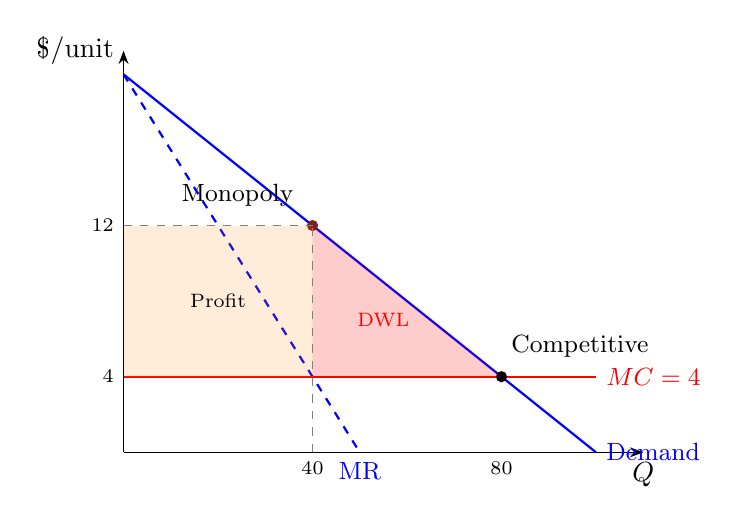
\begin{tikzpicture}[scale=0.6, >=Stealth]
  % Axes
  \draw[->] (0,0) -- (11,0) node[below] {$Q$};
  \draw[->] (0,0) -- (0,8.5) node[left] {\$/unit};
  % Demand: P = 20 - 0.2Q. Q 0-100 => x 0-10, P 0-20 => y 0-8
  \draw[thick, blue] (0,8) -- (10,0) node[right, font=\small] {Demand};
  % MR: P = 20 - 0.4Q. At Q=50 P=0
  \draw[thick, blue, dashed] (0,8) -- (5,0) node[below, font=\small] {MR};
  % MC = 4 => y = 1.6
  \draw[thick, red] (0,1.6) -- (10,1.6) node[right, font=\small] {$MC=4$};
  % Competitive: Q=80 (x=8), P=4 (y=1.6)
  \filldraw (8, 1.6) circle (3pt);
  \node[above right, font=\small] at (8, 1.8) {Competitive};
  % Monopoly: Q=40 (x=4), P=12 (y=4.8)
  \filldraw[UoERed] (4, 4.8) circle (3pt);
  \node[above left, font=\small] at (3.8, 5) {Monopoly};
  % Monopoly profit shading
  \fill[orange, opacity=0.15] (0,1.6) rectangle (4,4.8);
  \node[font=\scriptsize] at (2, 3.2) {Profit};
  % DWL triangle
  \fill[red, opacity=0.2] (4,4.8) -- (8,1.6) -- (4,1.6) -- cycle;
  \node[font=\scriptsize, text=red] at (5.5, 2.8) {DWL};
  % Dashed lines
  \draw[dashed, gray] (4,0) -- (4,4.8);
  \draw[dashed, gray] (0,4.8) -- (4,4.8);
  \node[below, font=\scriptsize] at (4,0) {$40$};
  \node[below, font=\scriptsize] at (8,0) {$80$};
  \node[left, font=\scriptsize] at (0,4.8) {$12$};
  \node[left, font=\scriptsize] at (0,1.6) {$4$};
\end{tikzpicture}
\end{center}
\vspace{0.3em}
The orange rectangle is monopoly profit (transferred from consumers).\\
The red triangle is \alert{deadweight loss} --- value destroyed, captured by no one.
\end{frame}

\begin{frame}{Synthesis: When Does the Invisible Hand Work?}
\begin{center}
\begin{tabular}{lccc}
\toprule
\textbf{Condition violated} & \textbf{Failure} & \textbf{Result}
  & \textbf{Policy} \\
\midrule
No externalities & Pollution & Overproduction & Pigouvian tax \\
Full information  & Adverse selection & Market collapse
  & Disclosure \\
Perfect competition & Monopoly & Under-production & Antitrust \\
\bottomrule
\end{tabular}
\end{center}
\vspace{0.5em}
\begin{alertblock}{The Mature View}
Neither ``markets always work'' nor ``markets never work'' survives
contact with computation. The question is always: \textit{which
conditions hold here, and what happens when they don't?}
\end{alertblock}
\end{frame}

% -------------------------------------------------------------
\section{Part III --- Exercises \& Discussion}
% -------------------------------------------------------------

\begin{frame}{Exercise 1: Carbon Tax Calibration}
A coal-fired power plant with:
\vspace{0.3em}
\begin{align*}
  P(Q) &= 50 - 0.5\,Q & &\text{(Inverse demand)} \\
  PMC(Q) &= 10 + 0.2\,Q & &\text{(Private marginal cost)} \\
  EMD(Q) &= 0.3\,Q & &\text{(External marginal damage)}
\end{align*}
\vspace{0.3em}
\begin{enumerate}
  \item[(a)] Find the free-market equilibrium ($P = PMC$) and the social
        optimum ($P = PMC + EMD$). Compute both quantities and prices.
  \item[(b)] Compute the optimal Pigouvian tax $\tau^* = EMD(Q_{\text{soc}})$.
        Verify it restores the social optimum.
  \item[(c)] Compute the deadweight loss from the unregulated market.
  \item[(d)] Plot demand, PMC, SMC, and PMC + tax on one graph.
        Shade the deadweight loss.
\end{enumerate}
\end{frame}

\begin{frame}{Exercise 2: Public Goods and the Free-Rider Problem}
\textbf{Setup:} $N = 10$ residents each choose contribution $g_i \geq 0$
to a shared park. Total provision $G = \sum g_i$.
\[
  u_i = (w - g_i) + \beta\sqrt{G}, \qquad w = 100,\ \beta = 20
\]

\begin{enumerate}
  \item[(a)] \textbf{Nash equilibrium:} each player maximises $u_i$ taking
        others' contributions as given. Show
        $g_i^* = \frac{\beta^2}{4N^2}$. Compute $G^{NE}$.
  \item[(b)] \textbf{Social optimum:} a planner maximises $\sum u_i$
        choosing a common $g$. Derive $g^{SO}$ and $G^{SO}$.
  \item[(c)] Compute the ratio $G^{NE}/G^{SO}$. By what factor does the
        voluntary mechanism underprovide?
  \item[(d)] Plot total provision and utility under both regimes as
        $N$ varies from 2 to 50. Does the free-rider problem get better
        or worse?
\end{enumerate}
\end{frame}

\begin{frame}{Exercise 3: Reflection --- One Economist, One Model}
A combined writing and coding exercise:
\vspace{0.5em}
\begin{enumerate}
  \item[(a)] \textbf{Choose one economist} from the course (Smith, Ricardo,
        Malthus, Marx, the Marginalists, Keynes, Solow, Nash, Lucas,
        Piketty, or Akerlof). Write 150--250 words explaining their
        key idea and why it mattered.
  \item[(b)] \textbf{Implement a computational model} of that idea.
        It need not be complex --- but it must produce a quantitative
        result or a plot.
  \item[(c)] \textbf{Discuss:} what does your model \textit{capture}
        about the idea, and what does it \textit{miss}? (100--150 words)
  \item[(d)] \textbf{Connect} your economist's idea to one issue in the
        world today. How does it help us think? How might it mislead?
\end{enumerate}
\end{frame}

% -------------------------------------------------------------
\section{Quiz}
% -------------------------------------------------------------

\begin{frame}{Conceptual Questions (Q1--Q5)}
\textbf{Q1.} The First Welfare Theorem requires:\\
\quad (b) No externalities, no market power, and complete information.
\vspace{0.3em}

\textbf{Q2.} A negative externality causes the free market to:\\
\quad (b) Overproduce the good.
\vspace{0.3em}

\textbf{Q3.} In Akerlof's lemons model, adverse selection occurs because:\\
\quad (b) Sellers with high-quality goods withdraw when price reflects
average quality.
\vspace{0.3em}

\textbf{Q4.} The Scottish Enlightenment's key contribution to economics:\\
\quad (b) Emphasis on empirical observation, scepticism, and systematic
reasoning.
\vspace{0.3em}

\textbf{Q5.} Which is \textit{not} required for the invisible hand?\\
\quad (d) All consumers must have equal income.
\end{frame}

\begin{frame}{Computational Questions (Q6--Q10)}
\textbf{Q6.} Social optimum quantity in the pollution model ($P = SMC$):\\
\quad (b) $Q \approx 51.4$.
\vspace{0.3em}

\textbf{Q7.} A Pigouvian tax corrects an externality by:\\
\quad (b) Setting tax $= EMC$ at the socially optimal quantity.
\vspace{0.3em}

\textbf{Q8.} Monopoly DWL with $Q_m = 40$, $P_m = 12$, $Q_c = 80$,
$MC = 4$:\\
\quad (a) $\frac{1}{2}(80-40)(12-4) = 160$.
\vspace{0.3em}

\textbf{Q9.} As $N$ increases in the public goods game, the ratio
$G^{NE}/G^{SO}$:\\
\quad (c) Decreases as $1/N^2$ --- free-riding gets worse.
\vspace{0.3em}

\textbf{Q10.} The recurring computational method throughout the course:\\
\quad (b) Root-finding and optimisation (\texttt{fsolve}, \texttt{minimize}).
\end{frame}

% -------------------------------------------------------------
\section{Key Takeaways}
% -------------------------------------------------------------

\begin{frame}{What We Learned This Week}
\begin{enumerate}
  \item Smith's invisible hand works \textbf{under specific conditions}:
        perfect competition, no externalities, complete information.
  \item \textbf{Externalities} cause overproduction; a Pigouvian tax
        equal to the marginal external cost restores efficiency.
  \item \textbf{Asymmetric information} can cause markets to unravel
        through adverse selection (Akerlof's lemons).
  \item \textbf{Monopoly power} leads to underproduction and deadweight
        loss --- a concern Smith himself raised in 1776.
  \item We can \textbf{compute} each market failure precisely: the gap
        between market outcome and social optimum, and the policy
        that closes it.
  \item The mature view: the question is not ``markets vs.\ government''
        but \textit{which conditions hold and what follows when they don't}.
\end{enumerate}
\end{frame}

\begin{frame}{Course Synthesis}
\begin{center}
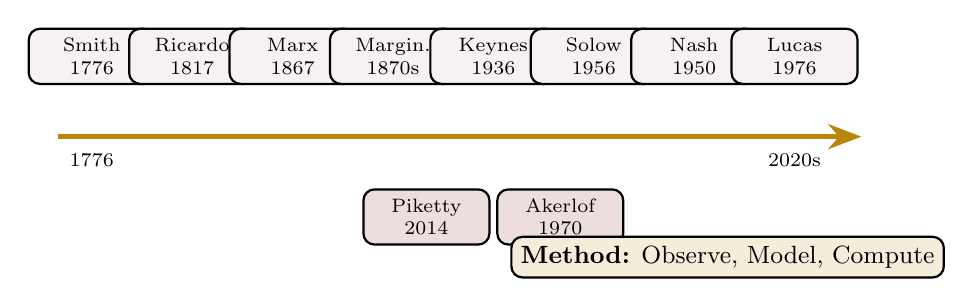
\begin{tikzpicture}[>=Stealth, thick, scale=0.85,
    mod/.style={draw, rounded corners, fill=UoERed!6,
                font=\scriptsize, minimum width=1.6cm,
                minimum height=0.7cm, align=center}]
  % Timeline
  \draw[->, UoEGold, line width=2pt] (-6,0) -- (6,0);
  % Modules
  \node[mod] at (-5.5, 1.2) {Smith\\1776};
  \node[mod] at (-4, 1.2)   {Ricardo\\1817};
  \node[mod] at (-2.5, 1.2) {Marx\\1867};
  \node[mod] at (-1, 1.2)   {Margin.\\1870s};
  \node[mod] at (0.5, 1.2)  {Keynes\\1936};
  \node[mod] at (2, 1.2)    {Solow\\1956};
  \node[mod] at (3.5, 1.2)  {Nash\\1950};
  \node[mod] at (5, 1.2)    {Lucas\\1976};
  \node[mod, fill=UoERed!15] at (-0.5, -1.2) {Piketty\\2014};
  \node[mod, fill=UoERed!15] at (1.5, -1.2)  {Akerlof\\1970};
  \node[below, font=\scriptsize] at (-5.5, -0.1) {1776};
  \node[below, font=\scriptsize] at (5, -0.1) {2020s};
  % Unifying theme
  \node[draw, rounded corners, fill=UoEGold!15, font=\small,
        minimum width=4cm] at (4, -1.8)
    {\textbf{Method:} Observe, Model, Compute};
\end{tikzpicture}
\end{center}
\vspace{0.3em}
Every module: an idea, a model, a computation.\\
The tools change; the commitment to evidence-based reasoning endures.
\end{frame}

\begin{frame}{Closing Reflection}
\begin{center}
\textit{``The real voyage of discovery consists not in seeking new
landscapes, but in having new eyes.''}\\[4pt]
--- Marcel Proust, \textit{In Search of Lost Time}
\end{center}
\vspace{1em}
\begin{itemize}
  \item The models are simple. Real economies are not.
  \item But the point of a model is not to replicate reality --- it is to
        \textbf{isolate a mechanism}, to make an idea precise enough to test.
  \item Computation gives us not answers, but \alert{sharper questions}.
  \item Economics is unfinished. The great questions remain open.
  \item But the method is clear: \textbf{Observe. Model. Compute. Test.
        Revise.}
  \item It is the method of Hume and Smith, updated for an age of data
        and code.
\end{itemize}
\end{frame}

\begin{frame}{Further Reading}
\begin{itemize}
  \item Akerlof, G. ``The Market for `Lemons'\,'' \textit{QJE} (1970).\\
        The paper that launched information economics.
  \item Pigou, A.\,C. \textit{The Economics of Welfare} (1920).\\
        The original treatment of externalities and corrective taxation.
  \item Nordhaus, W. \textit{The Climate Casino} (2013).\\
        Climate economics for a general audience.
  \item Broadie, A. \textit{The Scottish Enlightenment}.\\
        The intellectual world that made economics possible.
  \item Heilbroner, R. \textit{The Worldly Philosophers}.\\
        A magnificent tour through the lives and ideas of the great economists.
\end{itemize}
\vspace{1em}
\begin{center}
\textbf{End of course.}\\[4pt]
\textit{From Smith to Simulation --- The University of Edinburgh.}
\end{center}
\end{frame}

\end{document}
